\documentclass[11pt, twoside]{report}

\usepackage{fontspec}
\usepackage[utf8]{inputenc}
\usepackage[bitstream-charter]{mathdesign}
\usepackage{bbding}
\usepackage{ragged2e}
\usepackage{parskip}
\usepackage{enumitem}
\usepackage{titlesec}
\usepackage{paracol}
\usepackage{mdframed}
\usepackage[margin=1in]{geometry}

\usepackage[autocompile]{gregoriotex}

\titleformat{\chapter}[block]{\huge\scshape\filcenter}{}{1em}{}
\titleformat{\section}[block]{\Large\bfseries\filcenter}{}{1em}{}

\mdfsetup{skipabove=\topskip, skipbelow=\topskip}

\newcommand{\rubric}[1]{
	\switchcolumn[0] {
		\itshape
		#1
	}
}

\newcommand{\latinenglish}[2]{
	\switchcolumn[0]* {
		#1
	}
	\switchcolumn[1] {
		\itshape\small
		#2
	}
}

\newcommand{\latinenglishequal}[2]{
	\switchcolumn[0]* {
		#1
	}
	\switchcolumn[1] {
		\itshape
		#2
	}
}

\newenvironment{latinenglishsection}
	{\columnratio{.7, .3} \begin{paracol}{2}}
	{\end{paracol}}

\newenvironment{latinenglishequalsection}
	{\columnratio{.5, .5}\begin{paracol}{2}}
	{\end{paracol}}

\setlength{\columnseprule}{0.4pt}

\newcommand{\heading}[1]{
	\begin{leftcolumn}
		#1
	\end{leftcolumn}
}

\newcommand{\spanning}[1]{
	\switchcolumn*[#1]
}

\newenvironment{verses}[1]
	{\begin{flushleft} \begin{enumerate}[leftmargin=*] \setcounter{enumi}{#1}}
	{\end{enumerate} \end{flushleft}}

\newenvironment{versicles}{\par\leavevmode\parskip=0pt}{}

\newenvironment{collect}
{
	\leavevmode
	\parindent=1em
	\parskip=0pt
	\noindent Orémus.\par
}{}

\newenvironment{optionbox}
{
	\switchcolumn[0]
	\begin{mdframed}
%	\begin{minipage}{0.8\linewidth}
}{
%	\end{minipage}
	\end{mdframed}
}

\newcommand{\optionrule}{
	\begin{center}
	\rule{0.5\linewidth}{0.6pt}
	\end{center}
}

\newenvironment{optionruled}
{
	\optionrule
}
{
	\optionrule
}

% for use inside the collect environment
\newcommand{\Amen}{\par\noindent \Rbar. Amen.}

\begin{document}

\vspace*{4cm}

\begin{center}
	\textbf{\Huge Terce of the Blessed Virgin Mary}\\
	{\LARGE According to the Washtenaw Use}
\end{center}

\vspace*{1cm}
%\maketitle

%\begin{figure}[h!]
	%\centering
%\end{figure}

\begin{center}
	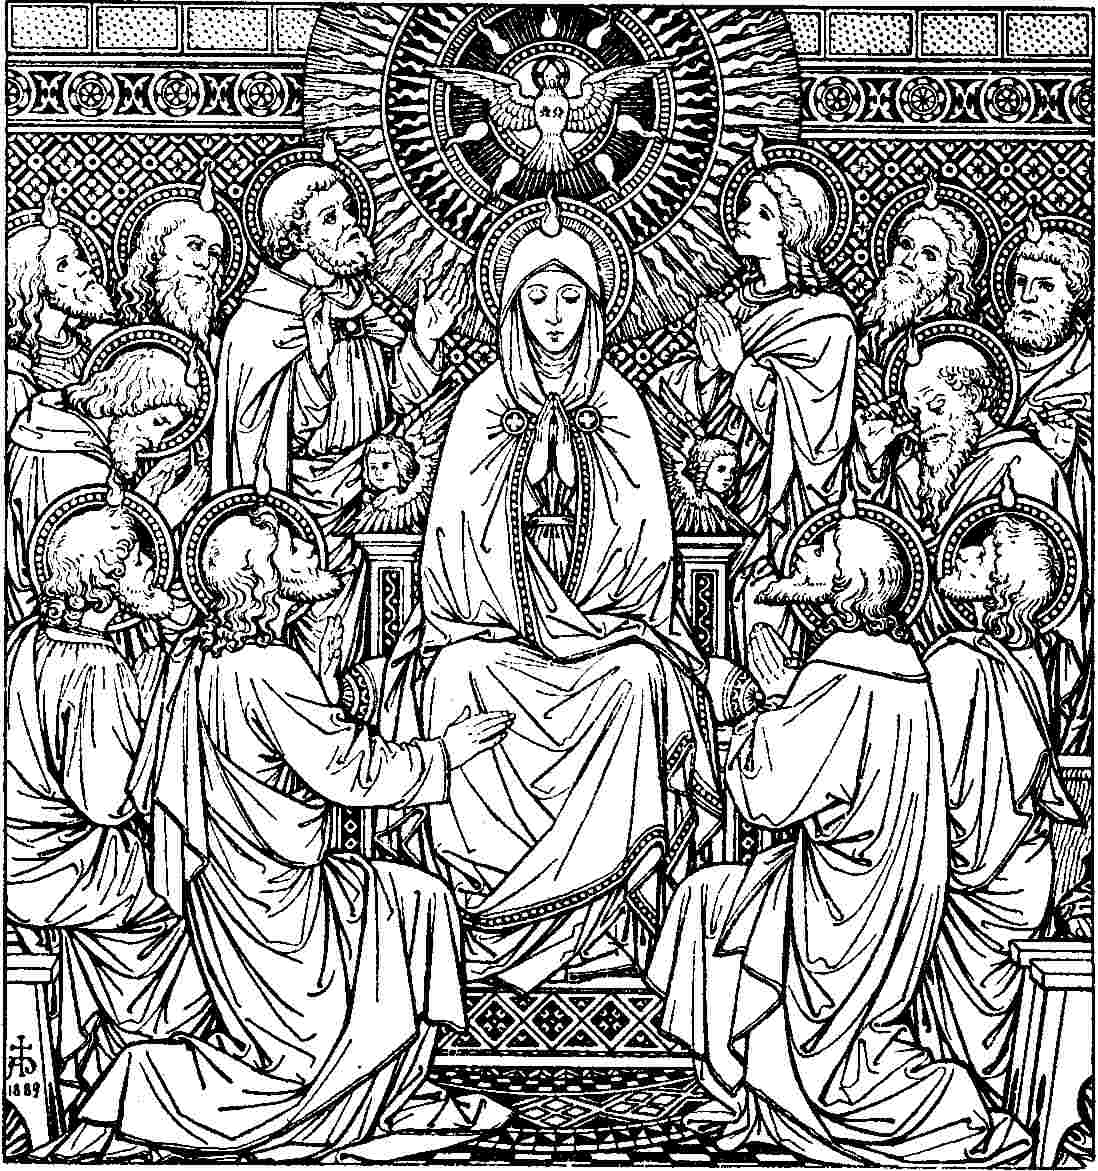
\includegraphics[width=0.8\textwidth]{Pentecost}
\end{center}

\hspace{0pt}
\vfill

\pagebreak

\vspace*{7.5cm}
``At the hour of \textit{Terce}, Our Lord Jesus Christ was scourged, crowned with thorns, and scorned. After His Resurrection, the same hour, He appeared to the women coming from the sepulchre. And on Pentecost Sunday, the same hour, He sent the Holy Ghost down to the Apostles and the Blessed Virgin.'' (Paraphrased from the \textit{Mirror of Our Lady}.) O most Blessed Virgin, your son was rejected and most cruelly treated, but He was vindicated by His rising from the sepulchre in glory; pray that we might experience in our lives the power of His Spirit. Amen.
\vfill

\pagebreak

\chapter*{Before Terce}

\section*{Preparatory Prayers}

\textit{All kneel and pray silently. As you say the prayer \textnormal{Aperi, Domine}, make the sign of the cross with your thumb first over your lips, and then over your heart.}

\begin{latinenglishequalsection}

\latinenglishequal{
	Áperi, {\color{red}\maltese}\ Dómine, os meum ad benedicéndum\linebreak nomen sanctum tuum:
	{\color{red}\maltese}\ munda quoque cor meum ab ómnibus vanis, pervérsis et aliénis cogitatiónibus;
	intelléctum illúmina, afféctum inflámma, ut digne, atténte ac devóte hoc Offícium beátæ Vírginis Maríæ recitáre váleam,
	et exaudíri mérear ante conspéctum divínæ Majestátis tuæ.
	Per Christum Dóminum nostrum. 
	Amen.
}{
	Open, {\color{red}\maltese}\ O Lord, my mouth to bless Thy holy Name; {\color{red}\maltese}\ cleanse also my heart from all vain, evil, and wandering thoughts; enlighten my understanding and kindle my affections; that I may worthily, attentively, and devoutly say this Office of the Blessed Virgin Mary, and so merit to be heard before the presence of Thy divine Majesty.  Through Christ our Lord.  Amen.
}

\latinenglishequal{
	Domine, in unióne illíus divínæ intentiónis, qua ipse in terris laudes Deo persolvísti, has tibi Horas persólvo.
}{
	O Lord, in union with that divine intention wherewith thou, whilst here on earth, didst render praises unto God, I desire to offer this my Office of prayer unto thee.
}

\latinenglishequal{
	Ave María, grátia plena, Dóminus tecum. Benedíc\-ta tu in muliéribus, et benedíctus fructus ventris tui, Jesus.
 Sancta María, Mater Dei, ora pro nobis peccatóribus, nunc et in hora mortis nostræ. Amen.
 }{
 	Hail Mary, full of grace, the Lord is with thee. Blessed art thou among women, and blessed is the fruit of thy womb, Jesus.
 Holy Mary, Mother of God, pray for us sinners, now and at the hour of our death. Amen.
 }
 
 \end{latinenglishequalsection}
 
\chapter*{Terce}

\begin{latinenglishsection}

\heading{\section*{Invitatory}}

\rubric{\color{red}All make the Sign of the Cross as the Officiant says the ``Deus in Adjutorium''. All continue together with the entire ``Gloria Patri'' after the response: }

\latinenglish{
	\gresetinitiallines{1}
	\gregorioscore{deus_in_adjutorium_minor}
}{
	O God, come to my assistance.
		
	O Lord, make haste to help me.
	
	Glory be to the Father, and to the Son, and to the Holy Spirit,
	as it was in the beginning, is now, and ever shall be, world without end. Amen.
	
	Alleluia.
}

\rubric{\color{red}From Septuagesima until Easter, \textnormal{Alleluia} is replaced with:}

\latinenglish{
	\gresetinitiallines{0}
	\gabcsnippet{
	(c3)Lau(h)s ti(h)bi(h) Dó(h)mi(h)ne(h), Re(h)x æ(h)té(h)rnæ(i) gló(h)ri(h)æ.(g) (::)
	}
}{
	Praise to thee, O Lord, King of everlasting glory.
}

\end{latinenglishsection}

\vfill\pagebreak

\begin{latinenglishsection}

\heading{\section*{Hymn}}

\latinenglish{
	\gresetinitiallines{0}
	\gregorioscore{memento_rerum_conditor}
}{
	1. Remember, Make of all things, 
	That once the form of our flesh, 
	From the Virgin's sacred womb, 
	Being born, Thou didst assume.
	
	2. Mary, Mother of grace, 
	Sweet parent of clemency, 
	Thou protect us from the enemy, 
	And receive us at the hour of death.
	
	3. Jesus, to Thee be glory, 
	Who wast born of the Virgin, 
	With the Father, and the loving Spirit, 
	Unto sempiternal ages. Amen.
}

\rubric{\color{red} For `Throughout the Year', \underline{see page 6}.}
\rubric{\color{red} For `Advent', \underline{see page 9}.}
\rubric{\color{red} For `Christmastide', \underline{see page 12}.}

\end{latinenglishsection}

\vfill\pagebreak

\section*{THROUGHOUT THE YEAR}

\begin{latinenglishsection}

\heading{\section*{Psalm 119}}

\rubric{\color{red}The Cantor intones the antiphon and leads the first Psalm verse to the star (*). All sit, while the Cantor's side finishes the first verse together. The Officiants side then says the second Psalm verse, with each side alternating thereafter. The remaining Psalms are intoned up to the asterisk by the Cantor, repeating the pattern of sitting and standing until the antiphon is said in full at the very end.}

\latinenglish{
	\gresetinitiallines{1}
	\gregorioscore{maria_virgo_intonation}
}{
	The Virgin Mary...
}

\latinenglish{
	\gresetinitiallines{0}
	\gregorioscore{psalm_119_1_8G}
	
	\begin{verses}{1}
	
	\item Dómine, líbera ánimam meam a lábiis in\textbf{í}quis,~* et a lin\textit{gua} \textit{do}\textbf{ló}sa.

	\item Quid detur tibi, aut quid apponátur \textbf{ti}bi~* ad lin\textit{guam} \textit{do}\textbf{ló}sam?
	
	\item Sagíttæ poténtis a\textbf{cú}tæ,~* cum carbónibus de\textit{so}\textit{la}\textbf{tó}riis.
	
	\item Heu mihi! quia incolátus meus prolongátus est:~{\color{red}\GreDagger}\ habitávi cum habitántibus \textbf{Ce}dar:~* multum íncola fuit á\textit{ni}\textit{ma} \textbf{me}a.
	
	\item Cum his, qui odérunt pacem, eram pa\textbf{cí}ficus:~* {\color{red}\textit{(stand)}} cum loquébar illis, impugná\textit{bant} \textit{me} \textbf{gra}tis.
	
	\item {\color{red}\textit{(bow)}} Glória Patri, et \textbf{Fí}lio,~* et Spirí\textit{tu}\textit{i} \textbf{Sanc}to.
	
	\item {\color{red}\textit{(rise)}} Sicut erat in princípio, et nunc, et \textbf{sem}per,~* et in s\'{\ae}cula sæcu\textit{ló}\textit{rum}. \textbf{A}men.
		
	\end{verses}
}{
	1. When I was in trouble I cried unto The Lord:
	and he heard me.
	
	2. O Lord, deliver my soul from wicked lips:
	and from a deceitful tongue.
	
	3. What can be given to thee, or what can be superadded to thee:
	unto a deceitful tongue?
	
	4. Sharp arrows of the mighty one:
	with desolating coals.
	
	5. Woe is me, that my sojourning is prolonged! I have dwelt with the inhabitants of Cedar:
	my soul hath been long a sojourner.
	
	6. With them that hated peace, I was peaceable:
	when I spake unto them, they fought against me without a cause.
	
	7. Glory be to the Father, and to the Son, and to the Holy Spirit:
	As it was in the beginning, is now, and ever shall be, world without end. Amen.
}

\end{latinenglishsection}

\vfill\pagebreak

\begin{latinenglishsection}

\heading{\section*{Psalm 120}}

\latinenglish{
	\gresetinitiallines{0}
	\gregorioscore{psalm_120_1_8G}
	
	\begin{verses}{1}
	
	\item Auxílium meum a \textbf{Dó}mino,~* qui fecit cæ\textit{lum} \textit{et} \textbf{ter}ram.

	\item Non det in commotiónem pedem \textbf{tu}um:~* neque dormítet \textit{qui} \textit{cus}\textbf{tó}dit te.
	
	\item Ecce, non dormitábit neque \textbf{dór}miet,~* qui cus\textit{tó}\textit{dit} \textbf{Is}raël.
	
	\item Dóminus custódit te, Dóminus protéctio \textbf{tu}a,~* super manum déx\textit{te}\textit{ram} \textbf{tu}am.
	
	\item Per diem sol non \textbf{u}ret te:~* neque lu\textit{na} \textit{per} \textbf{noc}tem.
	
	\item Dóminus custódit te ab omni \textbf{ma}lo:~* custódiat ánimam \textit{tu}\textit{am} \textbf{Dó}minus.
	
	\item Dóminus custódiat intróitum tuum, et éxitum \textbf{tu}um:~* {\color{red}\textit{(stand)}} ex hoc nunc, et us\textit{que} \textit{in} \textbf{s\'{\ae}}culum.
	
	\item {\color{red}\textit{(bow)}} Glória Patri, et \textbf{Fí}lio,~* et Spirí\textit{tu}\textit{i} \textbf{Sanc}to.
	
	\item {\color{red}\textit{(rise)}} Sicut erat in princípio, et nunc, et \textbf{sem}per,~* et in s\'{\ae}cula sæcu\textit{ló}\textit{rum}. \textbf{A}men.
	
	\end{verses}
}{
	1. I have lifted up mine eyes unto the hills:
	from whence shall come my help.
	
	2. My help is in the Lord: 
	who hath made heaven and earth.
	
	3. Let him not suffer thy foot to be moved:
	neither let him sleep that keepeth thee.
	
	4. Behold, he shall neither slumber nor sleep:
	that keepeth Israel.
	
	5. The Lord is thy keeper, the Lord is thy defense:
	upon thy right hand.
	
	6. The sun shall not burn thee by day:
	nor the moon by night.
	
	7. The Lord preserveth thee from all evil:
	may the Lord preserve thy soul.
	
	8. May the Lord preserve thy coming in and thy going out:
	from this time forth forever more.
	
	9. Glory be to the Father, and to the Son, and to the Holy Spirit:
	As it was in the beginning, is now, and ever shall be, world without end. Amen.
}

%\end{latinenglishsection}

%\begin{latinenglishsection}

\heading{\section*{Psalm 121}}

\latinenglish{
	\gresetinitiallines{0}
	\gregorioscore{psalm_121_1_8G}
	
	\begin{verses}{1}
	
	\item Stantes erant pedes \textbf{nos}tri,~* in átriis tu\textit{is}, \textit{Je}\textbf{rú}salem.

	\item Jerúsalem, quæ ædificátur ut \textbf{cí}vitas:~* cujus participátio ejus \textit{in} \textit{id}\textbf{íp}sum.
	
	\item Illuc enim ascendérunt tribus, tribus \textbf{Dó}mini:~* testimónium Israël ad confiténdum nó\textit{mi}\textit{ni} \textbf{Dó}mini.
	
	\item Quia illic sedérunt sedes in ju\textbf{dí}cio,~* sedes super \textit{do}\textit{mum} \textbf{Da}vid.
	
	\item Rogáte quæ ad pacem sunt Je\textbf{rú}salem:~* et abundántia dili\textit{gén}\textit{ti}\textbf{bus} te:
	
	\item Fiat pax in virtúte \textbf{tu}a:~* et abundántia in túr\textit{ri}\textit{bus} \textbf{tu}is.
	
	\item Propter fratres meos, et próximos \textbf{me}os,~* loquébar \textit{pa}\textit{cem} \textbf{de} te:
	
	\item Propter domum Dómini, Dei \textbf{nos}tri,~* {\color{red}\textit{(stand)}} quæsívi \textit{bo}\textit{na} \textbf{ti}bi.
	
	\item {\color{red}\textit{(bow)}} Glória Patri, et \textbf{Fí}lio,~* et Spirí\textit{tu}\textit{i} \textbf{Sanc}to.
	
	\item {\color{red}\textit{(rise)}} Sicut erat in princípio, et nunc, et \textbf{sem}per,~* et in s\'{\ae}cula sæcu\textit{ló}\textit{rum}. \textbf{A}men.
	
	\end{verses}
	
	\gresetinitiallines{1}
	\gregorioscore{maria_virgo}
}{
	1. I was glad at the things that were said unto me:
	We will go into the house of the Lord.
	
	2. Our feet were wont to stand:
	in thy courts, O Jerusalem.
	
	3. Jerusalem, which is built as a city:
	that is at unity with itself.
	
	4. For thither did the tribs go up, the tribes of the Lord:
	the testimony of Israel, to praise the Name of the Lord.
	
	5. For there are set the seats of judgement: 
	the seats over the house of David.
	
	6. Pray ye for the things that are for the peace of Jerusalem:
	and plenteousness be to the them that love thee.
	
	7. Let pece be in thy strength:
	and plenteousness in thy towers.
	
	8. For my brethren and companions' sake:
	I spake peace concerning thee.
	
	9. Because of the house of The Lord our God:
	I have sought good things for thee.
	
	10. Glory be to the Father, and to the Son, and to the Holy Spirit:
	As it was in the beginning, is now, and ever shall be, world without end. Amen.
	
	The Virgin Mary was taken up to the heavenly chamber, where the King of kings sitteth on his starry throne.
}

\rubric{\color{red}Proceed to page 15.}

\end{latinenglishsection}

\vfill\pagebreak

\section*{ADVENT}

\begin{latinenglishsection}

\heading{\section*{Psalm 119}}

\rubric{\color{red}The Cantor intones the antiphon and leads the first Psalm verse to the star (*). All sit, while the Cantor's side finishes the first verse together. The Officiants side then says the second Psalm verse, with each side alternating thereafter. The remaining Psalms are intoned up to the asterisk by the Cantor, repeating the pattern of sitting and standing until the antiphon is said in full at the very end.}

\latinenglish{
	\gresetinitiallines{1}
	\gregorioscore{ave_maria_intonation}
}{
	Hail Mary...
}

\latinenglish{
	\gresetinitiallines{0}
	\gregorioscore{psalm_119_1_1g}
	
	\begin{verses}{1}
	
	\item Dómine, líbera ánimam meam a lábi\textbf{is} in\textbf{í}quis,~* et a lin\textit{gua} \textit{do}\textbf{ló}sa.

	\item Quid detur tibi, aut quid appo\textbf{ná}tur \textbf{ti}bi~* ad lin\textit{guam} \textit{do}\textbf{ló}sam?
	
	\item Sagíttæ pot\textbf{én}tis a\textbf{cú}tæ,~* cum carbónibus de\textit{so}\textit{la}\textbf{tó}riis.
	
	\item Heu mihi! quia incolátus meus prolongátus est:~{\color{red}\GreDagger}\ habitávi cum habi\textbf{tán}tibus \textbf{Ce}dar:~* multum íncola fuit á\textit{ni}\textit{ma} \textbf{me}a.
	
	\item Cum his, qui odérunt pacem, \textbf{e}ram pa\textbf{cí}ficus:~* {\color{red}\textit{(stand)}} cum loquébar illis, impugná\textit{bant} \textit{me} \textbf{gra}tis.
	
	\item {\color{red}\textit{(bow)}} Glória \textbf{Pa}tri, et \textbf{Fí}lio,~* et Spirí\textit{tu}\textit{i} \textbf{Sanc}to.
	
	\item {\color{red}\textit{(rise)}} Sicut erat in princípio, et \textbf{nunc}, et \textbf{sem}per,~* et in s\'{\ae}cula sæcu\textit{ló}\textit{rum}. \textbf{A}men.
		
	\end{verses}
}{
	1. When I was in trouble I cried unto The Lord:
	and he heard me.
	
	2. O Lord, deliver my soul from wicked lips:
	and from a deceitful tongue.
	
	3. What can be given to thee, or what can be superadded to thee:
	unto a deceitful tongue?
	
	4. Sharp arrows of the mighty one:
	with desolating coals.
	
	5. Woe is me, that my sojourning is prolonged! I have dwelt with the inhabitants of Cedar:
	my soul hath been long a sojourner.
	
	6. With them that hated peace, I was peaceable:
	when I spake unto them, they fought against me without a cause.
	
	7. Glory be to the Father, and to the Son, and to the Holy Spirit:
	As it was in the beginning, is now, and ever shall be, world without end. Amen.
}

\end{latinenglishsection}

\vfill\pagebreak

\begin{latinenglishsection}

\heading{\section*{Psalm 120}}

\latinenglish{
	\gresetinitiallines{0}
	\gregorioscore{psalm_120_1_1g}
	
	\begin{verses}{1}
	
	\item Auxílium \textbf{me}um a \textbf{Dó}mino,~* qui fecit cæ\textit{lum} \textit{et} \textbf{ter}ram.

	\item Non det in commotiónem \textbf{pe}dem \textbf{tu}um:~* neque dormítet \textit{qui} \textit{cus}\textbf{tó}dit te.
	
	\item Ecce, non dormitábit \textbf{ne}que \textbf{dór}miet,~* qui cus\textit{tó}\textit{dit} \textbf{Is}raël.
	
	\item Dóminus custódit te, Dóminus pro\textbf{téc}tio \textbf{tu}a,~* super manum déx\textit{te}\textit{ram} \textbf{tu}am.
	
	\item Per diem \textbf{sol} non \textbf{u}ret te:~* neque lu\textit{na} \textit{per} \textbf{noc}tem.
	
	\item Dóminus custódit te ab \textbf{om}ni \textbf{ma}lo:~* custódiat ánimam \textit{tu}\textit{am} \textbf{Dó}minus.
	
	\item Dóminus custódiat intróitum tuum, et \textbf{éx}itum \textbf{tu}um:~* {\color{red}\textit{(stand)}} ex hoc nunc, et us\textit{que} \textit{in} \textbf{s\'{\ae}}culum.
	
	\item {\color{red}\textit{(bow)}} Glória \textbf{Pa}tri, et \textbf{Fí}lio,~* et Spirí\textit{tu}\textit{i} \textbf{Sanc}to.
	
	\item {\color{red}\textit{(rise)}} Sicut erat in princípio, et \textbf{nunc}, et \textbf{sem}per,~* et in s\'{\ae}cula sæcu\textit{ló}\textit{rum}. \textbf{A}men.
	
	\end{verses}
}{
	1. I have lifted up mine eyes unto the hills:
	from whence shall come my help.
	
	2. My help is in the Lord: 
	who hath made heaven and earth.
	
	3. Let him not suffer thy foot to be moved:
	neither let him sleep that keepeth thee.
	
	4. Behold, he shall neither slumber nor sleep:
	that keepeth Israel.
	
	5. The Lord is thy keeper, the Lord is thy defense:
	upon thy right hand.
	
	6. The sun shall not burn thee by day:
	nor the moon by night.
	
	7. The Lord preserveth thee from all evil:
	may the Lord preserve thy soul.
	
	8. May the Lord preserve thy coming in and thy going out:
	from this time forth forever more.
	
	9. Glory be to the Father, and to the Son, and to the Holy Spirit:
	As it was in the beginning, is now, and ever shall be, world without end. Amen.
}

%\end{latinenglishsection}

%\begin{latinenglishsection}

\heading{\section*{Psalm 121}}

\latinenglish{
	\gresetinitiallines{0}
	\gregorioscore{psalm_121_1_1g}
	
	\begin{verses}{1}
	
	\item Stantes erant \textbf{pe}des \textbf{nos}tri,~* in átriis tu\textit{is}, \textit{Je}\textbf{rú}salem.

	\item Jerúsalem, quæ ædifi\textbf{cá}tur ut \textbf{cí}vitas:~* cujus participátio ejus \textit{in} \textit{id}\textbf{íp}sum.
	
	\item Illuc enim ascendérunt tribus, \textbf{tri}bus \textbf{Dó}mini:~* testimónium Israël ad confiténdum nó\textit{mi}\textit{ni} \textbf{Dó}mini.
	
	\item Quia illic sedérunt sedes \textbf{in} ju\textbf{dí}cio,~* sedes super \textit{do}\textit{mum} \textbf{Da}vid.
	
	\item Rogáte quæ ad pacem \textbf{sunt} Je\textbf{rú}salem:~* et abundántia dili\textit{gén}\textit{ti}\textbf{bus} te:
	
	\item Fiat pax in vir\textbf{tú}te \textbf{tu}a:~* et abundántia in túr\textit{ri}\textit{bus} \textbf{tu}is.
	
	\item Propter fratres meos, et \textbf{pró}ximos \textbf{me}os,~* loquébar \textit{pa}\textit{cem} \textbf{de} te:
	
	\item Propter domum Dómini, \textbf{De}i \textbf{nos}tri,~* {\color{red}\textit{(stand)}} quæsívi \textit{bo}\textit{na} \textbf{ti}bi.
	
	\item {\color{red}\textit{(bow)}} Glória \textbf{Pa}tri, et \textbf{Fí}lio,~* et Spirí\textit{tu}\textit{i} \textbf{Sanc}to.
	
	\item {\color{red}\textit{(rise)}} Sicut erat in princípio, et \textbf{nunc}, et \textbf{sem}per,~* et in s\'{\ae}cula sæcu\textit{ló}\textit{rum}. \textbf{A}men.
	
	\end{verses}
	
	\gresetinitiallines{1}
	\gregorioscore{ave_maria}
}{
	1. I was glad at the things that were said unto me:
	We will go into the house of the Lord.
	
	2. Our feet were wont to stand:
	in thy courts, O Jerusalem.
	
	3. Jerusalem, which is built as a city:
	that is at unity with itself.
	
	4. For thither did the tribs go up, the tribes of the Lord:
	the testimony of Israel, to praise the Name of the Lord.
	
	5. For there are set the seats of judgement: 
	the seats over the house of David.
	
	6. Pray ye for the things that are for the peace of Jerusalem:
	and plenteousness be to the them that love thee.
	
	7. Let pece be in thy strength:
	and plenteousness in thy towers.
	
	8. For my brethren and companions' sake:
	I spake peace concerning thee.
	
	9. Because of the house of The Lord our God:
	I have sought good things for thee.
	
	10. Glory be to the Father, and to the Son, and to the Holy Spirit:
	As it was in the beginning, is now, and ever shall be, world without end. Amen.
	
	Hail Mary, full of Grace, The Lord is with thee. Blessed art thou amongst women. Alleluia.
}

\rubric{\color{red}Proceed to page 15.}

\end{latinenglishsection}

\vfill\pagebreak

\section*{CHRISTMASTIDE}

\begin{latinenglishsection}

\heading{\section*{Psalm 119}}

\rubric{\color{red}The Cantor intones the antiphon and leads the first Psalm verse to the star (*). All sit, while the Cantor's side finishes the first verse together. The Officiants side then says the second Psalm verse, with each side alternating thereafter. The remaining Psalms are intoned up to the asterisk by the Cantor, repeating the pattern of sitting and standing until the antiphon is said in full at the very end.}

\latinenglish{
	\gresetinitiallines{1}
	\gregorioscore{quando_natus_est_intonation}
}{
	In the bush...
}

\latinenglish{
	\gresetinitiallines{0}
	\gregorioscore{psalm_119_1_3a2}
	
	\begin{verses}{1}
	
	\item Dómine, líbera ánimam meam a lábi\textbf{is} in\textbf{í}quis,~* et a lin\textit{gua} \textit{do}\textbf{ló}sa.

	\item Quid detur tibi, aut quid appo\textbf{ná}tur \textbf{ti}bi~* ad lin\textit{guam} \textit{do}\textbf{ló}sam?
	
	\item Sagíttæ pot\textbf{én}tis a\textbf{cú}tæ,~* cum carbónibus de\textit{so}\textit{la}\textbf{tó}riis.
	
	\item Heu mihi! quia incolátus meus prolongátus est:~{\color{red}\GreDagger}\ habitávi cum habi\textbf{tán}tibus \textbf{Ce}dar:~* multum íncola fuit á\textit{ni}\textit{ma} \textbf{me}a.
	
	\item Cum his, qui odérunt pacem, \textbf{e}ram pa\textbf{cí}\textbf{fi}cus:~* {\color{red}\textit{(stand)}} cum loquébar illis, impugná\textit{bant} \textit{me} \textbf{gra}tis.
	
	\item {\color{red}\textit{(bow)}} Glória \textbf{Pa}tri, et \textbf{Fí}\textbf{li}o,~* et Spirí\textit{tu}\textit{i} \textbf{Sanc}to.
	
	\item {\color{red}\textit{(rise)}} Sicut erat in princípio, et \textbf{nunc}, et \textbf{sem}per,~* et in s\'{\ae}cula sæcu\textit{ló}\textit{rum}. \textbf{A}men.
		
	\end{verses}
}{
	1. When I was in trouble I cried unto The Lord:
	and he heard me.
	
	2. O Lord, deliver my soul from wicked lips:
	and from a deceitful tongue.
	
	3. What can be given to thee, or what can be superadded to thee:
	unto a deceitful tongue?
	
	4. Sharp arrows of the mighty one:
	with desolating coals.
	
	5. Woe is me, that my sojourning is prolonged! I have dwelt with the inhabitants of Cedar:
	my soul hath been long a sojourner.
	
	6. With them that hated peace, I was peaceable:
	when I spake unto them, they fought against me without a cause.
	
	7. Glory be to the Father, and to the Son, and to the Holy Spirit:
	As it was in the beginning, is now, and ever shall be, world without end. Amen.
}

\end{latinenglishsection}

\vfill\pagebreak

\begin{latinenglishsection}

\heading{\section*{Psalm 120}}

\latinenglish{
	\gresetinitiallines{0}
	\gregorioscore{psalm_120_1_3a2}
	
	\begin{verses}{1}
	
	\item Auxílium \textbf{me}um a \textbf{Dó}\textbf{mi}no,~* qui fecit cæ\textit{lum} \textit{et} \textbf{ter}ram.

	\item Non det in commotiónem \textbf{pe}dem \textbf{tu}um:~* neque dormítet \textit{qui} \textit{cus}\textbf{tó}dit te.
	
	\item Ecce, non dormitábit \textbf{ne}que \textbf{dór}\textbf{mi}et,~* qui cus\textit{tó}\textit{dit} \textbf{Is}raël.
	
	\item Dóminus custódit te, Dóminus pro\textbf{téc}tio \textbf{tu}a,~* super manum déx\textit{te}\textit{ram} \textbf{tu}am.
	
	\item Per diem \textbf{sol} non \textbf{u}\textbf{ret} te:~* neque lu\textit{na} \textit{per} \textbf{noc}tem.
	
	\item Dóminus custódit te ab \textbf{om}ni \textbf{ma}lo:~* custódiat ánimam \textit{tu}\textit{am} \textbf{Dó}minus.
	
	\item Dóminus custódiat intróitum tuum, et \textbf{éx}itum \textbf{tu}um:~* {\color{red}\textit{(stand)}} ex hoc nunc, et us\textit{que} \textit{in} \textbf{s\'{\ae}}culum.
	
	\item {\color{red}\textit{(bow)}} Glória \textbf{Pa}tri, et \textbf{Fí}\textbf{li}o,~* et Spirí\textit{tu}\textit{i} \textbf{Sanc}to.
	
	\item {\color{red}\textit{(rise)}} Sicut erat in princípio, et \textbf{nunc}, et \textbf{sem}per,~* et in s\'{\ae}cula sæcu\textit{ló}\textit{rum}. \textbf{A}men.
	
	\end{verses}
}{
	1. I have lifted up mine eyes unto the hills:
	from whence shall come my help.
	
	2. My help is in the Lord: 
	who hath made heaven and earth.
	
	3. Let him not suffer thy foot to be moved:
	neither let him sleep that keepeth thee.
	
	4. Behold, he shall neither slumber nor sleep:
	that keepeth Israel.
	
	5. The Lord is thy keeper, the Lord is thy defense:
	upon thy right hand.
	
	6. The sun shall not burn thee by day:
	nor the moon by night.
	
	7. The Lord preserveth thee from all evil:
	may the Lord preserve thy soul.
	
	8. May the Lord preserve thy coming in and thy going out:
	from this time forth forever more.
	
	9. Glory be to the Father, and to the Son, and to the Holy Spirit:
	As it was in the beginning, is now, and ever shall be, world without end. Amen.
}

%\end{latinenglishsection}

%\begin{latinenglishsection}

\heading{\section*{Psalm 121}}

\latinenglish{
	\gresetinitiallines{0}
	\gregorioscore{psalm_121_1_3a2}
	
	\begin{verses}{1}
	
	\item Stantes erant \textbf{pe}des \textbf{nos}tri,~* in átriis tu\textit{is}, \textit{Je}\textbf{rú}salem.

	\item Jerúsalem, quæ ædifi\textbf{cá}tur ut \textbf{cí}\textbf{vi}tas:~* cujus participátio ejus \textit{in} \textit{id}\textbf{íp}sum.
	
	\item Illuc enim ascendérunt tribus, \textbf{tri}bus \textbf{Dó}\textbf{mi}ni:~* testimónium Israël ad confiténdum nó\textit{mi}\textit{ni} \textbf{Dó}mini.
	
	\item Quia illic sedérunt sedes \textbf{in} ju\textbf{dí}\textbf{ci}o,~* sedes super \textit{do}\textit{mum} \textbf{Da}vid.
	
	\item Rogáte quæ ad pacem \textbf{sunt} Je\textbf{rú}\textbf{sa}lem:~* et abundántia dili\textit{gén}\textit{ti}\textbf{bus} te:
	
	\item Fiat pax in vir\textbf{tú}te \textbf{tu}a:~* et abundántia in túr\textit{ri}\textit{bus} \textbf{tu}is.
	
	\item Propter fratres meos, et \textbf{pró}ximos \textbf{me}os,~* loquébar \textit{pa}\textit{cem} \textbf{de} te:
	
	\item Propter domum Dómini, \textbf{De}i \textbf{nos}tri,~* {\color{red}\textit{(stand)}} quæsívi \textit{bo}\textit{na} \textbf{ti}bi.
	
	\item {\color{red}\textit{(bow)}} Glória \textbf{Pa}tri, et \textbf{Fí}\textbf{li}o,~* et Spirí\textit{tu}\textit{i} \textbf{Sanc}to.
	
	\item {\color{red}\textit{(rise)}} Sicut erat in princípio, et \textbf{nunc}, et \textbf{sem}per,~* et in s\'{\ae}cula sæcu\textit{ló}\textit{rum}. \textbf{A}men.
	
	\end{verses}
	
	\gresetinitiallines{1}
	\gregorioscore{quando_natus_est}
}{
	1. I was glad at the things that were said unto me:
	We will go into the house of the Lord.
	
	2. Our feet were wont to stand:
	in thy courts, O Jerusalem.
	
	3. Jerusalem, which is built as a city:
	that is at unity with itself.
	
	4. For thither did the tribs go up, the tribes of the Lord:
	the testimony of Israel, to praise the Name of the Lord.
	
	5. For there are set the seats of judgement: 
	the seats over the house of David.
	
	6. Pray ye for the things that are for the peace of Jerusalem:
	and plenteousness be to the them that love thee.
	
	7. Let pece be in thy strength:
	and plenteousness in thy towers.
	
	8. For my brethren and companions' sake:
	I spake peace concerning thee.
	
	9. Because of the house of The Lord our God:
	I have sought good things for thee.
	
	10. Glory be to the Father, and to the Son, and to the Holy Spirit:
	As it was in the beginning, is now, and ever shall be, world without end. Amen.
	
	When thou wast born of a Virgin, after an ineffable manner, then were the Scriptures fulfilled. Thou didst come down like rain upon the fleece, that thou mightest save mankind: we praise thee, O our God.
}

\rubric{\color{red}Proceed to the next page.}

\end{latinenglishsection}

\vfill\pagebreak

\begin{latinenglishsection}

\section*{The Little Chapter}

\rubric{\color{red}The Officiant leads the Little Chapter, which varies according to the season:}

\rubric{\textbf{Throughout the Year and in Christmastide:  Sirach 24:15}}

\latinenglish{
	Et sic in Sion firmata sum, {\color{red}\GreDagger}\ et in civitate sanctificata similiter \textit{requi}\textbf{e}vi, et in Jerusalem potestas mea.
	
	{\color{red}\Rbar.} Deo gratias.\\
	{\color{red}\Vbar.} Diffusa est gratia in labiis tuis.\\
	{\color{red}\Rbar.} Propterea benedixit te Deus in æternum.\\
	{\color{red}\Vbar.} Domine, exaudi orationem meam.\\
	{\color{red}\Rbar.} Et clamor meus ad te veniat.
}{
	And so was I established in Sion, and in the holy city likewise I rested, and my power was in Jerusalem.
	
	{\color{red}\Rbar.} Thanks be to God.
	{\color{red}\Vbar.} Grace was poured forth on thy lips.
	{\color{red}\Rbar.} Therefore hath God blessed thee forever.
	{\color{red}\Vbar.} O Lord, hear my prayer.
	{\color{red}\Rbar.} And let my cry come unto thee.
}

\end{latinenglishsection}

\begin{latinenglishsection}

\rubric{\textbf{In Advent: Isaiah 6:1-2}}

\latinenglish{
	Egredietur virga de radice Jesse, {\color{red}\GreDagger}\ et flos de radice e\textit{jus as}\textbf{cen}det. Et requiescet super eum Spiritus Domini.
	
	{\color{red}\Rbar.} Deo gratias.\\
	{\color{red}\Vbar.} Diffusa est gratia in labiis tuis.\\
	{\color{red}\Rbar.} Propterea benedixit te Deus in æternum.
}{
	The Lord God shall give unto him the throne of David his father: and he shall reign in the house of Jacob forever, and of his kingdom there shall be no end.
	
	{\color{red}\Rbar.} Thanks be to God.
	{\color{red}\Vbar.} Grace was poured forth on thy lips.
	{\color{red}\Rbar.} Therefore hath God blessed thee forever.
}

\end{latinenglishsection}

\vfill\pagebreak

\begin{latinenglishsection}

\section*{Collect}

\rubric{\color{red}The Officiant leads the concluding collect, which differs depending on the season:}

\rubric{\textbf{Throughout the Year and in Christmastide:}}

\latinenglish{
	Orémus.
	Deus, qui salutis æternæ, beatæ Mariæ virginitate foecunda, humano generi præmia præstitisti: {\color{red}\GreDagger}\ tribue, quæsumus; ut ipsam pro nobis intercedere \textit{senti}\textbf{a}mus, per quam meruimus auctorem vitæ\\ suscipere, ~* Dominum nnostrum Jesum Christum, Filium tuum. Qui tecum vivit et regnat in unitate Spiritu Sancti Deus, per omnia s\'{\ae}cula sæculórum.
	
	{\color{red}\Rbar.} Amen.
}{
	Let us pray.
	O God, who, by the fruitful virginity of the Blessed Mary, has given to mankind the rewards of eternal salvation; grant, we beseech thee, that we may be sensible of her intercession, through whom we have received the author of life, Our Lord Jesus Christ, Thy Son. Who liveth and reigneth in the unity of the Holy Spirit, world without end.
	
	{\color{red}\Rbar.} Amen.
}

\end{latinenglishsection}

\begin{latinenglishsection}

\rubric{\textbf{In Advent:}}

\latinenglish{
	Orémus.
	Deus, qui de beatæ Mariæ virginis utero Verbum tuum, Angelo nuntiante, carnem suscipere voluisti: {\color{red}\GreDagger}\ præsta supplicibus tuis, ut qui vere eam Genitricem De\textit{i cre}\textbf{di}mus, ejus apud te intercessionibus adjuvemur. ~* Per eumdem Dominum nostrum Jesum Christum filium tuum, Qui tecum vivit et regnat in unitate Spiritu Sancti Deus, per omnia s\'{\ae}cula sæculórum.
	
	{\color{red}\Rbar.} Amen.
}{
	Let us pray.
	O God, who wast pleased that thy Word, at the message of an Angel, should take flesh in the womb of the Blessed Virgin Mary; grant to us, thy humble servants, that, as we believe her to be truly the Mother of God, we may be assisted also by her intercessions with thee. Through the same Lord Jesus Christ thy Son, who liveth and reigneth with Thee in the unity of the Holy Spirit, world without end.
	
	{\color{red}\Rbar.} Amen.
}

\end{latinenglishsection}

\vfill\pagebreak

\begin{latinenglishsection}

\section*{Conclusion}

\rubric{\color{red} The Officiant leads the conclusion; the Benedicamus is that of the common tone, except when during Paschal time:}

\latinenglish{
	\gresetinitiallines{0}
	\gabcsnippet{(c3) <c><sp>V/</sp>.</c> Do(h)mi(h)ne(h) e(h)xau(h)di(h) o(h)ra(h)ti(h)ó(h)nem(h) me(h)am.(f) (::)}

	\gresetinitiallines{0}
	\gabcsnippet{(c3) <c><sp>R/</sp>.</c> Et(h) cla(h)mor(h) me(h)us(h) ad(h) te(h) vé(h)ni(h)at.(f) (::)}
}{
	{\color{red}\Vbar.} O Lord, hear my prayer.
	{\color{red}\Rbar.} And let my cry come unto thee.
}

\latinenglish{
	\gresetinitiallines{0}
	\gabcsnippet{(c3)<c><sp>V/</sp>.</c> Be(h)ne(h)di(h)cá(h)mus(h) Dó(f)mi(ef)no.(f.) (::)}
	
	\gresetinitiallines{0}
	\gabcsnippet{(c3)<c><sp>R/</sp>.</c> De(h)o(h) grá(f)ti(ef)as.(f.) (::)}
}{
	
	{\color{red}\Vbar.} Let us bless the Lord.
	{\color{red}\Rbar.} Thanks be to God.
}

\end{latinenglishsection}

\begin{latinenglishsection}

\rubric{\color{red}In Paschal Time:}

\latinenglish{
	\gresetinitiallines{0}
	\gregorioscore{benedicamus_paschal}
}{
	{\color{red}\Vbar.} Let us bless the Lord.
	{\color{red}\Rbar.} Thanks be to God.
}

\end{latinenglishsection}

\begin{latinenglishsection}

\rubric{\color{red} The Officiant says the following in a low recto tono:}

\latinenglish{
	\gresetinitiallines{0}
	\gabcsnippet{(c3) <c><sp>V/</sp>.</c> Fi(f)dé(f)li(f)um(f) á(f)ni(f)mæ(f) per(f) mi(f)se(f)ri(f)cór(f)di(f)am(f) De(f)i(f), re(f)qui(f)é(f)scant(f) in(f) pa(f)ce(f.). (::) <c><sp>R/</sp>.</c> Am(f.)en.(f.) (::)}
}{
	{\color{red}\Vbar.} May the souls of the faithful departed, through the mercy of God, rest in peace.
	{\color{red}\Rbar.} Amen.
}
	
\end{latinenglishsection}

\end{document}